\mychapter{Àlgebra}{Àlgebra}{
\includegraphics[width=3.1cm]{img-02/chap2.jpg}
	
	{\footnotesize Al Khwarizmi (780-850) }}
{chap:algebra}
 

\section{Operacions amb polinomis}
\vspace{-0.35cm}
\subsection{Identitats notables}
\vspace{-0.35cm}
\begin{theorybox}
	\begin{tabular}{ll}
	    \textbf{Quadrat d'una suma}: & $(a+b)^2 = a^2 + 2 ab+b^2$ \\
		\textbf{Quadrat d'una diferència}: & $(a-b)^2 = a^2 - 2 ab+b^2$\\
		\textbf{Suma per diferència}: & $(a+b)\cdot(a-b) = a^2 - b^2$ \\ [0.8ex]  
		\textbf{Quadrat d'un trinomi}: & $(a+b+c)^2 = a^2+b^2+c^2+2ab+2ac+2bc$		
	\end{tabular}
\end{theorybox}

\begin{mylist}
   
    	\exer  Desenvolupa les següents potències:
	    \begin{tasks}(3)
	      \task $\left(2{x} - 5{y}\right)^{2}$   
	      \task $\left(3{x} + \frac{y}{3}\right)^{2}$   
	      \task $\left(5^{2} - \frac{5}{x} \right)^{2}$
	       \task $\left(3{a} - {b}\right)^{2}$ 
	        \task $\left({a}^2 + {b}^{2}\right)^{2}$  
	         \task $\left(\frac{3y}{5} - \frac{2}{y}\right)^{2}$
	   \end{tasks}
   \answers[cols=1]{[$4x^2-20xy+25y^2$, $9x^2 +2xy+y^2/9$, $625-250+25/x^2$, $9a^2-6ab+b^2$, $a^4+2a^2b^2+b^4$, $9y^2/25 - 12/5+4/y^2$]}
   
    	\exer  Expressa com el quadrat d'una suma o d'una diferència les següents expressions algebraiques:
	    \begin{tasks}(3)
		   \task  $a^4 + 6a^2 + 9 $
		    \task  $9{x}^{2} - 6{x} + 1 $
		     \task  ${b}^{2} - 10{b} + 25$
		   \task  $4{y}^{2} + 12{y} + 9  $
		    \task  $a^4-2a^2+1$
		     \task  $y^{4} + 6{y}^{2} + 9$
	    \end{tasks}
    \answers[cols=1]{[$(a^2+3)^2$, $(3x-1)^2$, $(b-5)^2$, $(2y+3)^2$, $(a^2-1)^2$, $(y^2+3)^2$]}
   
   
   	\exer  Efectua aquests productes:
    \begin{tasks}(3)
     \task $(4x^{2} +3y)\cdot (4x^{2} -3y)$ \task $(2x^{2} +8)\cdot (2x^{2} -8)$  \task $(-x^{2} +3x)\cdot (x^{2} +3x)$
       \end{tasks}
   	\answers{[$16x^4-9y^2$, $4x^4-64$, $-x^4+9x^2$]}
\end{mylist}

 

\subsection{Divisió de polinomis}
\begin{theorybox}
	\begin{minipage}{0.7\textwidth}
		Per poder dividir $D(x):d(x)$ necessitam que el grau($D$)$\ge$grau($d$).
		
		\textbf{Comprovació}: Si dividim el dividend $D(x)$ entre el divisor $d(x)$, i obtenim el quocient $q(x)$ i el residu $r(x)$, s'ha de complir que 
		\begin{equation*}
		D(x) = q(x) \cdot d(x) + r(x)
		\end{equation*}
		
		Si $d(x)=x \pm a$ podem emprar la regla de \textbf{Ruffini}, sinó hem de fer la divisió en general.
	\end{minipage}
\hspace{0.5cm}
	\begin{minipage}{0.3\textwidth}
		\centering
		\videonw{46}{Divisió general}
		
		\videonw{47}{Divisió Ruffini}
	\end{minipage}
\end{theorybox}

\begin{resolt}[E]{
	\textbf{$(x^4+3x^3 - 4x+5):(x+2)$}
}

	Feim la divisió per la regla de Ruffini, recordant a posar 0 si falten potències de $x$.
	
	\begin{center}
		\begin{tabular}{l|lllll}	
		   & 1 & 3  & 0  & -4 & 5 \\
		-2 &   & -2	& -2 & 4 & 0 \\ \hline
		   & 1 & 1 & -2 & 0 & $\boxed{5}$
		\end{tabular} 
	\end{center}
	
	Llavors, el quocient és $q(x)=x^3+x^2-2x$ i el residu $r=5$.
\end{resolt} 
\vspace{0.75cm}

\begin{mylist}
\exer[1] Efectua les divisions de polinomis indicant quin \'{e}s el quocient i residu.
\begin{tasks}
	\task $6x^{5} -x^{4} -8x^{3} +15x^{2} -8x{\rm \; entre\; }2x^{2} -3x+2$
	\task $2x^{3} +2x+1{\rm \; entre\; }x^{2} -x+1$
	\task $ax^{4} +b{\rm \; entre\; }x-1$      
	\task $x^{9} -x^{8} +x^{7} -x^{6} +x^{5} -x^{4} +x^{3} -x^{2} +x-{\rm 1\; entre\; }x-1$  
\end{tasks}
\answers[cols=1]{[
	 $Q(x)=3x^{3}+4x^{2}-x+2$; $R(x)=-4$, 
	 $Q(x)=2x+2$;  $R(x)=2x-1$,      
    $Q(x)=a(x^{3}+ x^{2}+ x+ 1)$; $R(x)=a+b$,
       $Q(x)=x^{8}+ x^{6}+ x^{4}+ x^{2}+ 1$; $R(x)=0$
]}

	\exer  Divideix els següents polinomis:   
\begin{tasks}
	\task $2x^{4} -x^{2} -x+7$ entre $x^{2} +2x+4$.    
	\task $-10x^{3} -2x^{2} +3x+4$ entre $5x^{3} -x^{2} -x+3$
	\task $4x^{5} -6x^{3} +6x^{2} -3x-7$ entre $-2x^{3} +x+3$   
	\task $-8x^{5} -2x^{4} +10x^{3} +2x^{2} +3x+5$ entre $4x^{3} +x^{2} +x-1$ 
	\task $-6x^{5} +x^{2} +1$ entre $x^{3} +1$ 
\end{tasks}
\answers[cols=1]{[$Q=2x^2-4x-1$; $R=17x+11$, 
	$Q=-2$; $R=-4x^2+x+10$, 
	$Q=-2x^2+2$; $R=12x^2-5x-13$, 
	$Q=-2x^2+3$; $R=-3x^2+8$, 
	$Q=-6x^2$; $R=7x^2+1$
	]}


\exer  Utilitza la regla de \textit{Ruffini} per realitzar les següents divisions de polinomis:
\begin{tasks}(2)
	\task $-3x^{2} +x+1$ entre $x-1$  
	\task $x^{4} +2x^{3} -2x+1$ entre $x-2$
	\task $4x^{3} -3x^{2} -1$ entre $x+1$   
	\task $x^{3} -9x+1$ entre $x-3$ 
\end{tasks}
\answers[cols=1]{[$Q=-3x-1$; $R=-1$, 
	$Q=x^3+4x^2+8x+14$; $R=29$, 
	$Q=4x^2-7x+7$; $R=-8$, 
	$Q=x^2+3x$; $R=1$ 
	]}
 
\end{mylist}

\begin{theorybox}[Teorema del residu]
	El residu de la divisió $P(x):(x-a)$ coincideix amb el valor numèric del polinomi $P(a)$.
\end{theorybox}




\begin{example}
		Donat el polinomi $P(x)=x^2+2x+1$ es fàcil comprovar que $P(-1)=(-1)^2-2+1=0$. Aleshores, asseguram que la divisió $(x^2+2x+1):(x+1)$ és exacta, té residu zero.  
	\vspace{0.25cm}
\end{example}

\begin{mylist}
\exer  Aplica el teorema del residu per saber si les següents divisions són exactes o no:
\begin{tasks}(2)
	\task $\dfrac{x^{5} +7x^{4} -13x^{3} +5x^{2} -17x+5}{x-3} $ \task $\dfrac{x^{5} +x^{4} -3x^{3} +3x^{2} -4x+4}{x-2} $ \task $\dfrac{9x^{5} +7x^{4} -3x^{3} +5x^{2} -17x-1}{x-1} $ 
\end{tasks}
\answers{[$R=458$, $R=32$, $R=0$]}

 
 
 \exer  Troba un polinomi $q(x)$ tal que en dividir $p(x)=x^{6} +x^{4} +x^{2} +x+1$ entre $q(x)$ s'obtingui com a polinomi residu $r(x)=5x^{4} +5x^{2} +1$.  
 \answers{Per exemple $q(x)=p-r=x^6-4x^4-4x^2+x+1$ que donaria quocient 1.}
 
\exer  Troba dos polinomis tals que en dividir-los obtinguem $q(x)=x^{2} -x-3$ com a polinomi quocient i $r(x)=-3x^{2} -1$ com a residu. 
	\answers{$D=d\cdot q + r$. Per exemple, si ens inventam $d=2x+1$, obtenim $D=2x^3-4x^2-7x-4$}

\end{mylist}


\subsection{Factorització de polinomis}

\begin{mylist}
 
\exer  Analitza si els següents polinomis han sorgit del desenvolupament de potències de binomis, o trinomis, o d'un producte \textit{suma per diferència}. En cas afirmatiu expressa la seva procedència. 
 \begin{tasks}(3)  
 \task $x^{2} -6x+9$  \task $x^{4} +8x^{2} +16$  \task $x^{2} +\sqrt{20} \, xy+5y^{2} $ \task $x^{4} +2x^{3} +x^{2} +2x+1$
\task $x^{4} -2x^{3} +x^{2} +2x+1$  \task $x^{2} -36$  \task $5x^{2} +1$   \task $5x^{2} -11$ \task $x^{4} -3y^{2} $
\end{tasks}
\answers[cols=1]{[$(x-3)^2$, $(x^2+4)^2$, $(x+\sqrt{5}y)^2$, NO, NO, $(x+6)(x-6)$, NO, $(\sqrt{5}x+\sqrt{11})(\sqrt{5}x-\sqrt{11})$, $(x^2+\sqrt{3}y)(x^2-\sqrt{3}y)$]}

\exer  Factoritza els següents polinomis. Ajuda't traient factor comú i identificant possibles identitats notables.
\begin{tasks}(4)
	\task $x^{2} -8x$  	
	\task $4x^{2} -x-3$  
	\task $x^{3} -4x$  	
	\task $x^{3} +25x$
	\task $3x^3+6x^2+3x$
	\task $x^4 - 16$
	\task $4x^2 - 4x +1$
	\task $x^4 - 2x^3$
\end{tasks}
\answers[cols=1]{[$x(x-8)$, $(4x+3)(x-1)$, $x(x+2)(x-2)$, $x(x^2+25)$, $3x(x+1)^2$, $(x+2)(x-2)(x^2+4)$, $(2x-1)^2$, $x^3(x-2)$]}

\end{mylist}

\begin{theorybox}[Procediment per factoritzar un polinomi:]
	
	\video[4]{50}{Factoritzar polinomis}
	
	\textbf{1r} Puc treure factor comú alguna cosa?
	
	\textbf{2n} Puc identificar alguna identitat notable?
	
	\textbf{3r} Queda un polinomi de segon grau $P(x)=ax^2+bx+c$? $\rightarrow$ Resoldre l'equació de 2n grau amb la fórmula
	\begin{center}
	$x_{1,2}=\dfrac{-b\pm\sqrt{b^2-4ac}}{2a}$. La factorització és $P(x)=\mathbf{a}\cdot (x-x_1)\cdot (x-x_2)$ 

	 
\includegraphics[width=0.8cm]{img-02/warning}	\color{red}{No us oblideu de copiar el coeficient $\mathbf{a}$ davant de la factorització.}
	\end{center}
	
	\textbf{4t} En altre cas, factoritzar utilitzant la regla de \textbf{Ruffini}.
\end{theorybox}


\begin{mylist}


\exer[1] Factoritza els polinomis fent servir la regla de Ruffini (pensa a extreure factor com\'{u}       quan sigui necessari).
\begin{tasks}(2)
	\task  $p(x)=3x^{2} +9x+6$=                  
	\task  $p(x)=x^{5} -9x^{3} $=
	\task  $p(x)=4x^{3} +12x^{2} -4x-12$=     
	\task  $p(x)=-2x^{3} +2x^{2} +10x+6$=                        
	\task  $p(x)=x^{4} -x^{3} +8x^{2} -4x$=               
	\task  $p(x)=x^{3} -3x-2$=
	\task  $p(x)=2x^{3} -12x^{2} +6x+20$=       
	\task  $p(x)=x^{4} -2x^{3} -3x^{2} $=      
	\task  $p(x)=x^{3} +3x^{2} -6x-8$=
\end{tasks} 
\answers[cols=1]{[
		 $3(x+2)\cdot (x+1)$,    
		 $x^{3}\cdot(x+3)\cdot(x-3)$,     
	     $4(x+3)\cdot (x+1)\cdot (x-1)$,     
		 $-2(x+1)^{2}\cdot (x-3)$,       
		 $x\cdot (x^{3}-x^{2}+8x-4)$,     
		 ($x+1)^{2}\cdot (x-2)$,     
		 $2(x+1)\cdot(x-2)\cdot(x-5)$,     
		 $x^{2}\cdot(x+1)\cdot(x-3)$,          
		 $(x+4)\cdot(x+1)\cdot(x-2)$
]}

\end{mylist}
\begin{example}
	 	a) Resolem l'equació $3x^{2} +9x+6=0$, trobam solucions $x=-1$ i $x=-2$. Aleshores, la factorització és $p(x)=3\cdot(x+1)\cdot(x+2)$
	
	b) Treim factor comú $x^3$, $p(x)=x^3 \cdot(x^{2} -9)$, identificam una identitat notable (suma $\times$ diferència) i trobam la factorització $p(x)=x^3 \cdot(x+3)\cdot (x-3)$
\end{example}


\section{Fraccions algebraiques}
\vspace{-0.25cm}
\subsection{Simplificar fraccions}
\vspace{-0.25cm}
\begin{theorybox}[Per simplificar una fracció algebraica:]
	
		
	1r Factoritzam el numerador i el denominador
	
	2n Tatxam tots els factors (que es troben multiplicant) repetits en el numerador i el numerador.	
\end{theorybox}
\begin{warningbox}
	\begin{minipage}{0.65\textwidth}
	 	\malament
		$\dfrac{\cancel{x^2}-1}{\cancel{x^2}+2x+1} \xcancel{=} \dfrac{-1}{2x+1}$
		
		
		
		\be
		$\dfrac{x^2-1}{x^2+2x+1} = \dfrac{\cancel{(x+1)}\cdot(x-1)}{(x+1)^{\cancel{2}}}=
		\dfrac{x-1}{x+1}$	
		
		
	\end{minipage}
	\begin{minipage}{0.25\textwidth}
		\centering
		\videonw{51}{Fraccions algebraiques}
	\end{minipage} 
\end{warningbox}

\begin{mylist}
	
	
	\exer  Calcula què ha de valer $m$ perquè el valor numèric de l'expressió algebraica següent sigui $-2$ per a  $x = 0$.
	\[\dfrac{x^{3} -mx+4}{(x^{4} -1)(mx+2)} \] 
	\answers{Per a qualsevol valor de $m$}
 
		\exer  Simplifica, si és possible, les següents expressions: 
 \begin{tasks}(3)
	\task $\dfrac{x^{2} +4x}{x^{3} +3x^{2} -6x-8} $  
	\task $\dfrac{x^{2} -1}{x^{3} +3x^{2} -6x-8} $   
	\task $\dfrac{x^{2} -1}{x^{3} +x^{2} -6x} $ 
\end{tasks}	
\answers{[$\dfrac{x}{(x+1)(x-2)}$, $\dfrac{x-1}{(x-2)(x+4)}$, Igual]}
 
\exer  Simplifica les següents fraccions algebraiques:
\begin{tasks}(2)	
\task $\dfrac{3x^{2} -6x}{9x^{2} +15} $ 
\task $\dfrac{a^{3} -5a^{2} }{7a^{3} +4a^{2} } $ 
 \task $\dfrac{x^{2} y+3xy^{2} }{4xy} $  
 \task$\dfrac{2a^{2} b^{2} +3ab}{a^{3} b-ab} $
\end{tasks}
\answers{[$\dfrac{x(x+2)}{x^2+5}$, $\dfrac{a-5}{7a+4}$, $\dfrac{x+3y}{4}$, $\dfrac{2ab+3}{(a+1)(a-1)}$]}	
  
\end{mylist}
 
\subsection{Operar fraccions}

	\begin{theorybox}[Procediment per calcular el \textbf{min.c.m} de polinomis:]
		\textbf{1r}\, Factoritzam tots els polinomis. 
		
		\textbf{2n}\, Multiplicam factors comuns i no comuns amb el major exponent.
		
		Per exemple $\text{min.c.m}\left[x^2+2x, x^2, x+2\right]=\text{min.c.m}\left[x(x+2), x^2, x+2\right]=x^2\cdot(x+2)$
	\end{theorybox}
\begin{mylist}	
	\exer Calcula el mín.c.m dels següents polinomis
	\begin{tasks}(2)
		\task mín.c.m[$x$, $x(x+1)$, $x+1$] =
		\task mín.c.m[$x^2$, $x^3-x$, $x^2-1$] =
		\task* mín.c.m[$x-2$, $x^2-2x+1$, $x^2-3x+2$] =
	\end{tasks}
\answers{[$x(x+1)$, $x^2(x+1)(x-1)$, $(x-1)^2 (x-2)$]}
	

	\exer[1] Opera i simplifica les fraccions algebraiques
	\begin{tasks}(2)
		\task $\dfrac{x}{3x+3} \cdot \dfrac{x^{2} -1}{x^{3} +2x^{2} } =$  
		\task $\dfrac{2x}{x+1} :\dfrac{x^{2} +x}{x+5} =$      
		\task $\dfrac{x}{x+1} :\dfrac{x^{2} +2x^{2} }{x^{2} -1} =$
		\task $\dfrac{x^{2} -1}{x+2} \cdot \dfrac{3x+1}{x^{2} +3} =$      
		\task $\dfrac{x^{2} +x+1}{x+1} :\dfrac{x}{x^{2} -1} =$    
		\task $\dfrac{1}{x^{2} -4} :\dfrac{1}{2-x} $
		\task  $\dfrac{x^{2} +2x}{x^{2} -1} \cdot \dfrac{x+1}{x} $  
		\task $\dfrac{2x}{x-1} :\dfrac{x^{3} }{x^{5} -1} $
	\end{tasks}
	\answers[cols=1]{[ 
			 $\dfrac{x-1}{3x(x+2)} $,   $\dfrac{2(x+5)}{(x+1)^{2} } $,     $\dfrac{x-1}{x(x+2)} $,    \textit{No es pot},    $\dfrac{(x^{2} +x+1)(x-1)}{x^{} } $,           $\dfrac{1}{x+2} $,         $\dfrac{x+2}{x-1} $,        $\dfrac{2(x^{4} -x^{3} +x^{2} -x+1)}{x} $]}
	
	
		\exer  Realitza les següents operacions tenint en compte les factoritzacions dels denominadors:
		\begin{tasks}(2)
	\task $\dfrac{5}{-3x+12} +\dfrac{x+2}{x^{2} -4x} $  
	\task $\dfrac{-x}{x^{2} -2x+1} -\dfrac{3x-1}{x^{2} -1} $
\end{tasks}
\answers{[$\dfrac{-2x+6}{3x(x-4)}$, $\dfrac{-4x^2+3x-1}{(x-1)^2 (x+1)}$]}


\end{mylist}
\begin{example}
	a) Factoritzam els denominadors $-3 x+12 = -3(x-4)$, $x^2-4x=x(x-4)$, el mím.c.m=$3\cdot x\cdot (x-4)$ que és el denominador comú.
	
	$\dfrac{5}{-3(x-4)} +\dfrac{x+2}{x(x-4)} = \dfrac{-5x}{3\cdot x\cdot (x-4)}+\dfrac{3(x+2)}{3\cdot x\cdot (x-4)}  $  
	
	finalment, operam i simplificam el numerador
	$= \dfrac{-5x+3 x+6}{3\cdot x\cdot (x-4)} = \dfrac{-2 x+6}{3\cdot x\cdot (x-4)} $  
	
\end{example}

\begin{mylist}

		\exer  Efectua els següents càlculs: 
	\begin{tasks}(2)
	\task $\dfrac{2x+1}{x^{2} +1} +\dfrac{4}{x} $ 
	 \task $\dfrac{1}{x-2} +\dfrac{3}{x+1} $  
	  \task $\dfrac{-x}{x^{2} +3x} \cdot \dfrac{1}{x-1} $ 
	   \task $\dfrac{x-2}{x^{2} +3x} :\dfrac{x-2}{x+3} $
\end{tasks}
\answers{[$\dfrac{6x^2+2x+4}{x(x^2+1)}$, $\dfrac{4x-5}{(x-2)(x+1)}$, $\dfrac{-1}{(x+3)(x-1)}$, $\dfrac{x+3}{x^2+3}$]}


		\exer  Realitza les següents operacions modificant, a cada apartat, únicament un dels denominadors, i el seu respectiu numerador: 
	\begin{tasks}(2)
		\task $\dfrac{-x^{2} +x-1}{x^{3} } -\dfrac{3x+2}{x^{2} } $  
		 \task $\dfrac{x-2}{x^{2} +3x} -\dfrac{8}{x+3} $
	\end{tasks}
\answers{[$-\dfrac{(4x^2+x+1)}{x^3}$, $-\dfrac{(7x+2)}{x(x+3)}$]}

\exer[1] Opera les fraccions algebraiques (\textit{ajuda: cercau el m.c.m. i redu\"{i}u a denominador com\'{u}})
\begin{tasks}(2)
	\task  $\dfrac{1+x}{1-x} -\dfrac{1-x}{1+x} =$   
	\task   $\dfrac{2}{x^{2} -1} -\dfrac{1}{x+1} -\frac{1}{x-1} =$ 
	\task $\dfrac{2(x-3)}{x^{2} +2x-3} -\dfrac{3}{x+3} =$  
	\task   $\dfrac{1}{t} +\dfrac{1-t}{t^{2} +2t} -\dfrac{2}{t+2} =$
	\task  $\dfrac{2x+6}{x} -\dfrac{2x^{2} +4x-6}{x^{2} -x} =$      
	\task   $x^{4} -(1-x^{2} )^{2} -2x^{2} +\dfrac{1}{x^{2} } =$
	\task  $\left(\dfrac{1}{x} -1\right)\cdot \left(\dfrac{4}{\left(1+x\right)^{2} } -\dfrac{x+1}{x-1} +\dfrac{x}{x+1} \right)=$  
\end{tasks}
\answers[cols=1]{[ $\dfrac{-4x}{(x+1)(x-1)} $,   $\dfrac{-2}{x+1} $,     $\dfrac{-1}{x-1} $,    $\dfrac{-2t+3}{t(t+2)} $,    0,     $\dfrac{1-x^{2} }{x^{2} } $,   $\dfrac{3x^{2} +5}{x(x+1)^{2} } $]}

\exer  Efectua les següents operacions i simplifica tot el possible:
\begin{tasks}(2)
	\task $\dfrac{\dfrac{1}{a} -\dfrac{1}{x-y} }{\dfrac{1}{a} +\dfrac{1}{x+y} } :\dfrac{\dfrac{1}{x} -\dfrac{1}{a+y} }{\dfrac{1}{x} +\dfrac{1}{a-y} } $ 
		\task $\dfrac{\dfrac{3}{x} +\dfrac{2}{y} }{\dfrac{1}{x} +\dfrac{3}{y} } \cdot \dfrac{\dfrac{2}{x} -\dfrac{1}{y} }{\dfrac{3}{x} +\dfrac{5}{y} } $ 
	\task* $\left(1-\dfrac{1}{x} -\dfrac{3}{x^{2} } +\dfrac{2}{x^{3} } \right):\left(\dfrac{1}{x} -\dfrac{3}{x^{2} } -\dfrac{2}{x^{3} } \right)$  
\end{tasks}
\answers[cols=1]{[$\dfrac{-(a+y)(x+y)(a+x-y)}{(a-y)(x-y)(a+x+y)}$, $\dfrac{(2x+3y)(2y-x)}{(3x+y)(5x+3y)}$, $\dfrac{(x-2)(x^2+x-1)}{x^2-3x-2}$]}

\end{mylist}



\section{Equacions}
\vspace{-0.5cm}
\begin{minipage}{0.8\textwidth}
	\subsection{Equacions polinòmiques}
\end{minipage}
\begin{minipage}{0.1\textwidth}
	\centering
	\videonw{52}{}
\end{minipage}

\begin{mylist}
	

	\exer  Per a cadascun dels següents polinomis assenyala, en primer lloc, quins nombres enters són candidats a ésser arrels seves i, després, determina quins  són:   
	\begin{tasks}(2)
		\task $x^{3} -x^{2} +2x-2$      \task $x^{4} +4x^{3} +4x^{2} +4x+3$   
		\task $2x^{3} +x^{2} -18x-9$    \task $x^{4} +2x^{3} +3x^{2} +6x$   
	\end{tasks}
		
\answers{a) $1, –1, 2, –2$; Arrel $x = 1$.\par b) $1, –1, 3, –3$; Arrels: $–3$ i $–1$. \par c) $1, –1, 3, –3, 9, –9$; Arrels: 2 i 1; \par d) $0, 1, –1, 2, –2, 3, –3, 6, –6$; Arrels 0 i $–2$.}

 
	\exer  Resoleu:  	
	\begin{tasks}(2) 
		\task$\frac{x^{2} }{25} +\frac{(x+3)^{2} }{9} =1$ 
		\task $\frac{x^{2} }{16} =1+\frac{3/4x}{9} $ 
		\task $4x^4+8x^2-12=0$
		 \task $80x^{4} -48x^{2} -12=0$ 
	\end{tasks}

	\textit{Ajuda}: Els apartats c) i d) són \textbf{equacions biquadrades}; és a dir, fent el canvi $x^2=t$ es transforma en una equació de 2n grau.
	
	\answers[cols=1]{[$x=-\dfrac{75}{17}$ i $x=0$, $x=\frac{2\pm 2\sqrt{37}}{3}$, $x=\pm 1$, $x=\pm \sqrt{\dfrac{3\pm \sqrt{24}}{10}}$]}

 	
\exer[1] Resol les equacions traient factor com\'{u} i factoritzant el polinomi 
\begin{tasks}(2)
	\task  $x^{4} +x^{3} -6x^{2} -4x+8=0$ 
	\task  $3x^{3} -75x=0$
	\task  $x(x+1)=2$   
	\task $x^{3} +6=\frac{4x^{3} +7x^{2} -2x}{x+2} $
	\task  $x(x^{2} -5x-13)+77=\frac{60}{x} $ 
	\task  $x^{3} -1=0$
	\task  $x^{3} +x^{2} -4x-4=0$ 
	\task  $x^{4} +3x^{3} -3x^{2} -11x-6=0$
	\task  $x^{3} -4x^{2} -4x+16=0$ 
	\task  $x^{4} +6x^{3} +9x^{2} -4x-12=0$
	\task  $x^{4} -13x^{2} +36=0$  
	\task $x^{2} (x-4)=5x$
\end{tasks}
\answers[cols=2]{[ 
		 $x=1,\,2,\,-2$,        $x=0,\,5,\,-5$,              $x=1,\,-2$,         $x=\pm2,\,3,\,-1$,
		  $x=1,\,3,\,5,\,-4$,    $x=1$,                  $x=-2,\,-1,\,2$,             $x=-3,\,-1,\,2$,
		   $x=-2,\,2,\,4$,      $x=-3,\,-2,\,1$,       $x=-3,\,3,\,-2,\,2$,   $x=-1,\,0,\,5$
]}

 \exer  Conjectura, i després demostra, una llei que ens permeti saber quan un polinomi qualsevol 
\[a_{n} x^{n} +a_{n-1} x^{n-1} +......+a_{1} x+a_{0} \] admet el nombre 0 com arrel.
\answers{No pot tenir terme independent, és a dir, $a_0=0$.}

\exer  Troba una regla que demostri quan un polinomi qualsevol $a_{n} x^{n} +a_{n-1} x^{n-1} +......+a_{1} x+a_{0}$ admet al número 1 com a arrel.
\answers{La suma de tots els coeficients ha d'ésser zero, és a dir, $a_n + a_{n-1}+\cdots+a_1+a_0=0$.}


\exer  Sumant set unitats al doble d'un nombre més els 3/2 del mateix obtenim com resultat el sèxtuple d'aquest nombre menys 23. De quin nombre es tracta?
\answers{El nombre és 12. $2x+7+3/2x=6x-23$}

\exer  Les dimensions d'un rectangle són 54 i 36 m. Traça una paral·lela al costat que mesura 36 m de manera que es formi un rectangle semblant al primer. Quines són les longituds dels segments en què aquesta paral·lela divideix al costat de 54 m?
\answers{Les dimensions són 30 m i 24 m. Planteig: $\dfrac{36}{54}=\dfrac{x}{36}$. }

\end{mylist}


\subsection{Equacions amb denominadors}

\begin{theorybox}[Procediment per eliminar els denominadors:]
	
	\textbf{1r} Factoritzam tots els denominadors i cerca el seu min.c.m. 
	
	\textbf{2n} Multiplicam tots els termes de l'equació pel min.c.m i simplificam.
\end{theorybox}

\begin{mylist}
	\exer Resol
	\begin{tasks}(2)
		\task $\dfrac{2x-4}{3x-2} =\dfrac{4}{7} $   \task $\dfrac{x+8}{x-1} -\dfrac{x+4}{x+1} =\dfrac{12x}{x^{2} -1} $   \task* $\dfrac{3(2x+1)}{4} -\dfrac{5x+3}{6} +4x+\dfrac{x+1}{3} =x+\dfrac{151}{12} $
	\end{tasks}
\answers{[$x=6$, $x=2$, $x=3$]}
	
\exer[1] Resol  
\begin{tasks}(2)
	\task $\dfrac{1-x}{6} +\dfrac{x-1}{3} =\dfrac{2x^{2} -1}{2} $  
	\task  $\dfrac{2x}{x-1} +\dfrac{1}{x} =\dfrac{13x+1}{3x} $
	\task $\dfrac{1}{x+1} +\dfrac{1}{x} =\dfrac{5}{6} $   
	\task  $\dfrac{x}{x+1} +\dfrac{2}{x-1} =3$
\end{tasks}
\answers[cols=2]{[ 
		 $x= \dfrac{2}{3},\,-\dfrac{1}{2}$,  $x=2,\,\dfrac{1}{7}$,  $x=2,\,-\dfrac{3}{5}$,  $\dfrac{1\pm \sqrt{41}}{4}$]}
 
\exer  Resoleu les equacions següents:
\begin{tasks}(3)
	\task $\dfrac{3x-1}{2x-4} =\dfrac{5}{9} $   \task $\dfrac{x}{2} +5=\dfrac{3x}{6} -7$   \task $\dfrac{5}{x+1} =\dfrac{5x}{x-1} -2$
\end{tasks}
\answers{[$x=-\dfrac{11}{17}$, $x=S.S.$, $x=S.S.$]}
\end{mylist}

\subsection{Equacions amb arrels quadrades}

\begin{theorybox}[
	Procediment per resoldre equacions amb arrels quadrades:]
	
	\video{54}{}
	
	\textbf{1r} Aïllam una de les arrels a un membre de l'equació. 
	
	\textbf{2n} Elevam cada membre al quadrat (anant en compte amb les identitats notables).
	
	El procés 1-2 elimina només \textbf{una} arrel. Hem de repetir el procés tantes vegades com arrels tingui l'equació.
	
	\textbf{IMPORTANT: Cal sempre comprovar les solucions}
\end{theorybox}

\begin{mylist}
\exer[1] Resol les seg\"{u}ents equacions i comprova les solucions:
\begin{tasks}(2)
	\task $\sqrt{x} +1=3$  
	\task $x=\sqrt{x}+2 $   
	\task $\sqrt{x+4} =3$
	\task $\sqrt{x+2} +4 =x$  
	\task $\sqrt{x+2} =x$   
	\task $\sqrt{\sqrt{x+2} } =14$
	\task $\sqrt{\sqrt{x-1} +1} =2$  
	\task $\sqrt{x+1} +\sqrt{x-2} =3$  
	\task $\sqrt{x-2} =\sqrt{x+5} -1$
	\task $\sqrt{x+7} -1=\sqrt{x-4} {\rm \; }$ 
	\task $\sqrt{x+2} =x-\sqrt{x+86}$ 
	\task $\sqrt{10-x} -\sqrt{x+3} =x$
\end{tasks}
\answers[cols=2]{[
		 $x=4$,     $x=4$,     $x=9$,    $x=7$,    $x=2$,     $x=38414$,    $x=10$,     $x=3$,     $x=11$,    $x=29$,   $x=14$,    $x=1$]}

\end{mylist}

\begin{example}
	d) $\sqrt{x+2} +4 =x$.
	
	Aïllam l'arrel $\sqrt{x+2} =x-4$, elevam al quadrat els dos membres
	
	$(\sqrt{x+2})^2 =(x-4)^2$, desenvolupam  $x+2 = x^2 - 8x + 16$ i arreglam l'equació de segon grau
	$x^2-9x+14=0$. Resolem l'equació de 2n grau amb la fórmula i obtenim $x=2$ i $x=7$.  Si comprovam les solucions dins l'equació \emph{original} veim que només $x=7$ és vàlida.
\end{example}

\pagebreak

\subsection{Sistemes d'equacions}
\begin{mylist}
\exer[1] Resol els sistemes lineals
\begin{tasks}(2)
	\task $\left\{\begin{array}{l} {5y-3x=72+5x} \\ {15x=y-1} \end{array}\right. \; $    
	\task  $\left\{\begin{array}{l} {x+2y=22} \\ {5(x-5)=y-3} \end{array}\right. \; $  
	\task  $\left\{\begin{array}{l} {x+y=12} \\ {x-y=8} \end{array}\right. \; $      
	\task  $\left\{\begin{array}{l} {x+y=11} \\ {x-y=-3} \end{array}\right. \; $  
	\task $\left\{\begin{array}{l} {3(x+y)-1=5x-4y} \\ {2x+3(y+1)=x+3(x+y-1)} \end{array}\right. \; $  
	\task  $\left\{\begin{array}{l} {4(x-1)-3(y+2)=-5y+x} \\ {5(x+3)=2y-3(y+x)+7} \end{array}\right. \; $
\end{tasks}
\answers[cols=2]{[
		 $x=1; y=16$,      $x=6; y=8$,      $x=10; y=2$,      $x=4; y=7$,     $x=3; y=1$,     $x=-2; y=8$
]}
 
\exer Resol els sistemes no lineals
\begin{tasks}(2)
\task  $\left\{\begin{array}{l} {x+y-xy=7} \\ {x-y-xy=-1} \end{array}\right. $       
\task  $\left\{\begin{array}{l} {2x-y+1=0} \\ {x^{2} +3xy=0} \end{array}\right. $ 
\task  $\left\{\begin{array}{l} {(x^{2} +1)\; y^{2} =5} \\ {4x-y=0} \end{array}\right. $             
\task  $\left\{\begin{array}{l} {\sqrt{x} +\sqrt{y} =5} \\ {\sqrt{x} -\sqrt{y} =1} \end{array}\right. $ 
\end{tasks}
\answers[cols=1]{[ $x=-1; y=4$,     $x=-\dfrac{3}{7}; y=\dfrac{1}{7}$ i $x=0; y=1$,     $x=-\dfrac{1}{2}; y=-2$ i $x=\dfrac{1}{2}; y=2$,     $x=9; y=4$    ]}

\end{mylist}

\section{Sistemes d'equacions lineals $n\times n$}

\subsection{Sistemes escalonats}
\begin{theorybox}
	Un sistema $3\times 3$ és \textbf{escalonat} si una equació conté només una incògnita, i en una altra en falta alguna de les altres dues incògnites.
	
	Això fa que el sistemes escalonats siguin molt fàcils de resoldre.
\end{theorybox}
\begin{mylist}
	 
\exer[1] Reconeix com sistemes escalonats i resol: 
\begin{tasks}(2)
	\task  $\left\{\begin{array}{llll} x &  & & =7 \\ 2x& -3y & &=8 \\ 3x& +y& -z&=12 \end{array}\right. $       
	\task  $\left\{\begin{array}{llll} 3x&+4y&&=0 \\ &2y&&=-6 \\ 5x&+y&-z&=17 \end{array}\right. $ 
	\task  $\left\{\begin{array}{llll} 3x&&&=-3 \\ &5y&&=20 \\ 2x&+y&-z&=-2 \end{array}\right. $        
	\task  $\left\{\begin{array}{llll} &y&&=4 \\ x&&-z&=11 \\ &y&-z&=7 \end{array}\right. $ 
\end{tasks}
\answers[cols=1]{[
		 $x=7; y=2; z=11$, 
		 $x=4; y=-3; z=0$, 
		 $x=-1; y=4; z=4$, 
		 $x=8; y=4; z=-3$ ]}

\exer[1] Resol els seg\"uents sistemes escalonats: 
\begin{tasks}(2)
	\task  $\left\{\begin{array}{llll} &y& &=-5 \\ &&2z&=8 \\ 3x&&&=3 \end{array}\right. $       
	\task  $\left\{\begin{array}{llll} x&+2y&-z&=-3 \\ 3x&+y&&=-5 \\ &5y&&=-10 \end{array}\right. $ 
	\task  $\left\{\begin{array}{llll} x&-5y&+3z&=8 \\ &3y&-z&=5 \\ &&4z&=4 \end{array}\right. $        
	\task  $\left\{\begin{array}{llll} 4x&+y&-z&=7 \\ &2y&&=8 \\ 3x&&&=9 \end{array}\right. $ 
\end{tasks}
\answers[cols=1]{[
		 $x=1; y=-5; z=4$, 
		 $x=-1; y=-2; z=-2$,
		 $x=15; y=2; z=1$, 
		 $x=3; y=4; z=9$ 
]}

\subsection{Mètode de Gauss}

\begin{theorybox}
	El mètode de Gauss aconsegueix transformar un sistema que no és \textbf{escalonat} en un equivalent i que sí ho és. Les transformacions permeses són:
	
	\begin{itemize}
		\item Canviar l'ordre de les equacions
		\item Multiplicar o dividir tota l'equació per un nombre.
		\item A una equació sumar-li una altra prèviament multiplicada per un nombre.
	\end{itemize}
	\begin{minipage}{0.5\textwidth}
		\centering
	 \videonw{136}{Resolució de sistemes pel mètode de Gauss}
	\end{minipage}
	\begin{minipage}{0.5\textwidth}
		\centering
			\videonw{137}{Classificació de sistemes 3x3 per Gauss}	
	\end{minipage}
	

\end{theorybox}


 \exer[1] Resol pel mètode de Gauss
 \begin{tasks}(2)
 	\task  $\left\{\begin{array}{ll} x+y+z&=2 \\ x-y+z&=6 \\ x-y-z&=0 \end{array}\right. $       
 \task  $\left\{\begin{array}{ll} 2x+3y&=14 \\ x-2y+z&=-3 \\ 2x-y-z&=9 \end{array}\right. $ 
 \task  $\left\{\begin{array}{ll} 5x-4y+3z&=9 \\ 2x+y-2z&=1 \\ 4x+3y+4z&=1 \end{array}\right. $        
 \task  $\left\{\begin{array}{lll} 2x-5y&+4z&=-1 \\ 4x-5y&+4z&=3 \\ 5x&-3z&=13 \end{array}\right. $ 
 \end{tasks}
\answers[cols=1]{[
		 $x=1; y=-2; z=3$, 
		 $x=4; y=2; z=-3$, 
		 $x=1; y=-1; z=0$, 
		 $x=2; y=\dfrac{1}{5}; z=-1$ 
]}
 
 \exer  Resoleu pel mètode de  Gauss  els sistemes:
  \begin{tasks}(2)
\task $\left\{\begin{array}{rl} 4x+2y-z&=5 \\ 5x-3y+z&=3 \\ 2x-y+z&=3 \end{array}\right. $ 
\task $\left\{\begin{array}{rl} x+y+z&=0 \\ 7x+2y-z&=0 \\ 3x+5y+4z&=0 \end{array}\right. $
  \end{tasks}
\answers[cols=1]{[
	$x=\dfrac{16}{15}; y=\dfrac{8}{5}; z=\dfrac{39}{15}$, 
	$x=0; y=0; z=0$ 
	]}

\exer  Resol els següents sistemes pel mètode de Gauss i discuteix el resultat:
 \begin{tasks}(3)
\task $\left\{\begin{array}{ll} x+y+2z&=4 \\ x+y&=2 \\ \quad \,\, y+z&=2 \end{array}\right. $   
\task $\left\{\begin{array}{rl} x+y+t&=3 \\ x+z-t&=1 \\ y+z+t&=3 \\ x-y+z&=1 \end{array}\right. $   
 \task $\left\{\begin{array}{rl} x-y+2z&=4 \\ 2x+y+5z&=13 \\ x+y-4z&=-6 \end{array}\right. $ 
\task $\left\{\begin{array}{rl} 3x+4y-z&=6 \\ 6x-6y+2z&=2 \\ x-y+2x&=-2 \end{array}\right. $   
\task $\left\{\begin{array}{rl} x+4y-8z&=-8 \\ 4x+8y-2z&=-2 \\ 8x-y-4z&=-4 \end{array}\right. $   
\task $\left\{\begin{array}{rl} x-2y+3z+4t&=6 \\ 2x-y+z-t&=1 \\ x-y+3z+2t&=5 \\ 3x-y+2z-3t&=1 \end{array}\right. $
  \end{tasks}
\answers[cols=1]{[
	$x=1; y=1; z=1$, 
	$x=1; y=1; z=1; t=1$, 
	$x=1; y=1; z=2$, 
	$x=\dfrac{5}{9}; y=\dfrac{11}{3}; z=\dfrac{31}{3}$
	$x=0; y=0; z=1$, 
	$x=1; y=1; z=1; t=1$
	]}

	\exer  Discuteix i resol, si és possible, el següent sistema:
	$\left\{\begin{array}{ll} x+2y-z&=1 \\ 2x+y-2z&=2 \\ x-y-z&=1 \end{array}\right.$ 
	\answers{Sistema compatible indeterminat:\par $x=\lambda; y=0; z=\lambda-1$}
	
	\exer  Discuteix i resol, quan sigui possible, els següents sistemes  lineals d'equacions.
   \begin{tasks}(2)
	\task $\left\{\begin{array}{ll} x-6y-4z&=-7 \\ x+8y+4z&=6 \\  x+y&=1 \end{array}\right.$
	
	\task $\left\{\begin{array}{ll} x+y-6z-4t&=6 \\ 3x+2y-3z+8t&=-7 \\ 3x-y-6z-4t&=2 \\ 4x-y+3z+12t&=0 \end{array}\right.$ 
	\end{tasks}
\answers{Els dos sistemes són incompatibles.}

 
\begin{theorybox}
	Els sistemes es classifiquen segons el nombre de solucions en:
	\begin{center}
		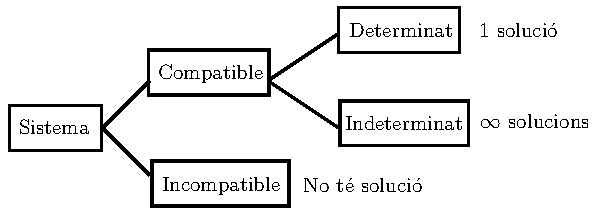
\includegraphics[width=10cm]{img-02/classificacio-sistemes.pdf}
	\end{center}

Si en aplicar el mètode de Gauss obtenim una fila de zeros $(0 0 0 | 0)$, el sistema serà compatible indeterminat (SCI). Si obtenim  una fila com  $(0 0 0 | a)$ serà incompatible (S.I.).
\end{theorybox}

 \exer \key{t2-key43} Resol pel mètode de Gauss i classifica en compatible determinat, compatible indeterminat o incompatible.
\begin{tasks}(2)
	\task  $\left\{\begin{array}{ll} x-y&=1 \\ 2x+6y-5z&=-4 \\ x+y-z&=0 \end{array}\right. $       
\task  $\left\{\begin{array}{ll} x+2y+z&=3 \\ x-2y+5z&=5 \\ 5x+22y+17z&=1 \end{array}\right. $ 
\task  $\left\{\begin{array}{ll} x+y+3z&=2 \\ 2x+3y+4z&=1 \\ -2x-y-8z&=-7 \end{array}\right. $        
\task  $\left\{\begin{array}{ll} 2x-y-z&=2 \\ 3x-2y-2z&=2 \\ -5x+3y+5z&=-1 \end{array}\right. $ 
\task  $\left\{\begin{array}{ll} x+y+z&=3 \\ -x+2y+z&=5 \\ x+4y+3z&=1 \end{array}\right. $ 
\task  $\left\{\begin{array}{ll} -2x+y+z&=1 \\ 3x+2y-z&=0 \\ -x+4y+z&=2 \end{array}\right. $ 
\end{tasks}



\exer  Desitgem vendre un cotxe, un pis i una finca per un total de 300000\euro. Si la finca val 4 vegades més que el cotxe i el pis cinc vegades més que la finca. Què val cada cosa?
\answers{Cotxe 12000 \euro{}; Finca 48000 \euro{}; Pis 240000 \euro{}}
 
	\exer  Una mare té el doble de la suma de les edats dels seus fills. L'edat del fill menor és la meitat de la seva germana. La suma de les edats dels nens i la de la mare és 45 anys. Quines edats tenen?
	\answers{$x-2y-2z=0$,\par $y-2z=0$,\par $x+y+z=45$.\par Solució: $x=30$, $y=10$, $z=5$ anys}
	 
	
	\exer  Les tres xifres d'un nombre sumen 18.  Si a aquest nombre se li resta el que resulta d'invertir l'ordre de les seves xifres, s'obté 594; la xifra de les desenes és mitja aritmètica entre les altres dues. Troba aquest nombre.
	\answers{$x+y+z=18$,\par $-99x+99z=594$,\par $y=(x+z)/2$.\par  Solució: $x=3$, $y=6$, $z=9$}
	
	
	\exer  Volem esbrinar les edats d'una família formada pels pares i els dos fills. Si sumam les seves edats de tres en tres, obtenim 100, 73, 74 i 98 anys, respectivament. Quina és l'edat de cadascun d'ells?
	\answers{$x+y+z=100$,\par $y+z+t=73$,\par $x+z+t=74$,\par $x+y+t=98$.\par Solució: $x=42$, $y=41$, $z=17$ i $t=15$ anys.}

\end{mylist}
 
\section{Inequacions}

\begin{theorybox}
	
	\video{61}{}
	
	\textbf{La solució d'una inequació es dóna en forma d'INTERVAL.}
	
	\textbf{Recorda:} Quan canviam els signes d'una inequació el sentit de la desigualtat canvia.
	
	Per exemple  $-4x + 1 > 9$, aïllam $-4x > 9-1$, i canviam els signes i el símbol $4x < -8$, que ens duu a $x<-2$, és a dir la semi-recta  $x\in (-\infty, -2)$.
\end{theorybox}

\begin{mylist}
\exer  Resol les següents inequacions i representa la solució a la recta real:
 \begin{tasks}(2)
\task $5 + 3{x} < 2{x} + 4 $
\task $3 + 4{x} \leq 8{x} + 6$ 
\task $4(3 + 2{x}) < -(6{x} + 8)$  
\task $7(2 + 3{x}) \leq 5(6{x} + 3)$
 \task $9(2 + 4{x}) + 4(5{x} - 2) > 3(2{x} + 1)$ 
 \end{tasks}
\answers{[$(-\infty,-1)$, $[9/4,+\infty)$, $(-\infty,x-10/7)$, $[-1/9,+\infty)$, $(-7/50,+\infty)$]}
 
\exer  Resol les següents inequacions i representa la solució a la recta real:
  \begin{tasks}(2)
\task $6 + 3{x} < {x}/3 + 1 $
\task $5 + 5{x}/2 \leq 9{x}/2 + 1$  
\task $(2 + 5{x})/3 > 4{x} + 1  $
\task $(1 + 5{x})/2 + 1 \geq (3{x} + 6)/4$
 \end{tasks}
  \answers{[$(-\infty,-1)$, $[2,+\infty]$, $(-\infty,-1/7)$, $[0,+\infty)$]}

 
\exer  Calcula els valors de  $x$ perquè sigui possible calcular les següents arrels:
  \begin{tasks}(2)
\task $\sqrt{2x-3} $  \task $\sqrt{-x-9} $  \task $\sqrt{2-7x} $   \task $\sqrt{-2x+7} $
 \end{tasks}
  \answers{[$[3/2,+\infty)$, $(-\infty,-9]$, $(-\infty,2/7]$, $(-\infty,7/2]$]}

\end{mylist}

\begin{example}
	\textbf{Inequacions de segon grau} 
	
	 $x^2-1 \ge 0$. Per resoldre una inequació de 2n grau, primer resoldrem l'equació canviant la desigualtat per un igual. $x^2-1 = 0$ té dues solucions $x=-1, x=1$. 
	
	\begin{center}
		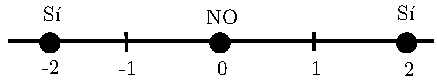
\includegraphics[width=6.5cm]{img-02/inequacion2ngrau.pdf}
	\end{center}
	La recta real ens queda divida en 3 trossos: $(-\infty,-1)$, $(-1,1)$, $(1,+\infty)$. Agafam un nombre qualsevol de cadascun dels intervals i comprovam si verifica l'inequació original $x^2-1 \ge 0$. Veim que el primer i darrer trossos són vàlids i el del mig no serveix.
	
	La solució és  $[-\infty,-1]\cup[1,+\infty]$. Hem escrit interval tancat perquè la desigualtat és major o igual.
\end{example}	
 	 
 \begin{mylist}
 		 
 	 
\exer  Resol les següents inequacions de segon grau:
  \begin{tasks}(3)
 \task $x^2-9>0$ 
 \task ${x}^{2} + 4 \ge 0$
\task $2{x}^{2} - 50 < 0$  
\task $3{x}^{2} +12 \le  0$    
\task $5{x}^{2} - 45 > 0$  
\task ${x}^{2 }+ 1 \ge  0$
 \end{tasks}
\answers[cols=1]{[$(-\infty,-3)\cup(3,+\infty)$, $\Re$, $(-5,5)$, $\emptyset$, $(-\infty,-3)\cup (3,+\infty)$, $\Re$]}

\end{mylist}



\begin{mylist}

 
\exer  Resol les següents inequacions de segon grau:
  \begin{tasks}(3)
\task $x^{2} + {x} \le 0  $ 
\task $x^{2} - 5{x} > 0 $  
\task $x^{2 } \le  8{x}$
	\task $x^{2} - 2{x} - 3 \le  0$
    \task ${-x}^{2}-2{x} + 8 \ge  0$
     \task $x^{2 }+ 9{x} + 14 > 0$
%      \task $x^{2} - 6{x} + 9 \le  0$
%\task $-x^{2 }-4{x} - 5 < 0$  
%\task $x^{2 }+ 8{x} + 16 > 0$    
 \end{tasks}

\answers[cols=1]{[$[-1,0]$, $(-\infty,0)\cup (5,+\infty)$, $[0,8]$, $[0,3]$, $(-\infty,0)\cup (3/2,+\infty)$, $(0,2)$]}
 
  \exer Per a quins valors de $x$ és possible obtenir les següents arrels?
 \begin{tasks}(4)
 	\task $\sqrt{x^{2} -1} $   \task $\sqrt{-x^{2} +4} $   \task $\sqrt{x^{2} +5x+6} $  \task $\sqrt{x^{2} -5x+6} $
 \end{tasks}
\answers[cols=1]{[$[-1,3]$, $[-4,2]$, $(-\infty,-7)\cup (-2,+\infty)$, $x=3$, $\Re$, $\Re$]}


\exer  Resol gràficament els següents sistemes d'inequacions:
  \begin{tasks}(2)
\task $\left\{\begin{array}{c} {\frac{1}{2} -\frac{x-2y+3}{3} \ge \frac{x-y+1}{2} } \\ {1-\frac{2x-4-y}{3} +\frac{2x+3y}{2} \ge 0} \end{array}\right. $  
 \task $\left\{\begin{array}{c} {x+y\ge 1} \\ {y-2x\ge 3} \\ {y\le 5} \end{array}\right. $  
 \task $\left\{\begin{array}{c} {x+y\ge 0} \\ {2x-y\ge 0} \\ {x\le 6} \end{array}\right. $  
 \task $\left\{\begin{array}{c} {(x+1)\cdot 10+x\le 6(2x+1)} \\ {4(x-10)<-6(2-x)-6x} \end{array}\right. $
 \end{tasks}
\answers{Solució gràfica:
	\par
	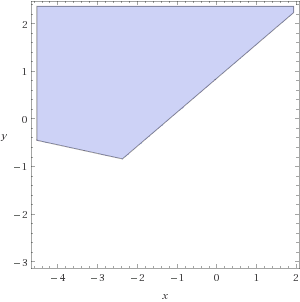
\includegraphics[width=0.3\textwidth]{img-sol/t2-55a}
	\par
	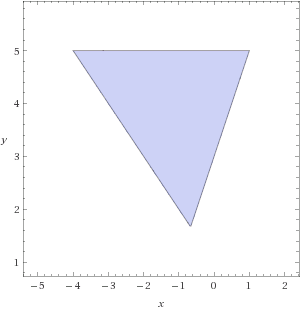
\includegraphics[width=0.3\textwidth]{img-sol/t2-55b}
	\par
	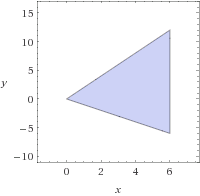
\includegraphics[width=0.3\textwidth]{img-sol/t2-55c}
	\par
	 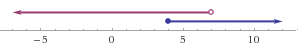
\includegraphics[width=0.4\textwidth]{img-sol/t2-55d}
}

\begin{comment}
\exer  Representa la regió factible del sistema:
\[\left\{\begin{array}{l} {x\ge 0} \\ {y\ge 0} \\ {6x+5y\le 30} \\ {x+2y\le 8} \end{array}\right. \] 
\end{comment}
\end{mylist}

\vspace{1cm}
 
\begin{autoaval}{31}

\begin{mylist}
	\exer[2] Quin és el valor numèric de l'expressió $\dfrac{3x-7}{2-3y^{2} } +5xy^{3} -\dfrac{6}{z} $ \par en $x=2,\, \, y=-1,\, \, z=-1$ ? 
\begin{comment}
  \begin{tasks}(4)
\task 17  \task 15   \task $-$3   \task $-$5
 \end{tasks}
\end{comment}
\answers{$-3$}
 
		\exer[2]  Divideix el polinomi $p(x)=x^{5} +x^{4} +x^{3} +1$ entre $q(x)=x^{2} +x+1$.
\begin{comment}
	  \begin{tasks}(2)
	 \task ha de ser de grau 2.    \task pot ser de grau 2. 
\task ha de ser de grau menor que 2.  \task cap de les opcions anteriors.
 \end{tasks}
\end{comment}
\answers{$Q=x^3$; $R=1$}

 
\exer[2]  És possible que un polinomi, amb coeficients enters, de grau quatre tingui exactament tres arrels reals, ja siguin diferents o amb alguna múltiple?  
\answers{No, si és de grau 4 pot tenir 4 arrels, que poden esser 4 reals, o be 2 arrels reals i 2 complexes o totes 4 complexes.} 
	
 
 
\exer[2]  Resol la inequació $x^{2} \leq 4$  
 \begin{comment}
   \begin{tasks}(2)
  \task {x} $\in$  ($-$2, 2)  \task {x}$\in$ [$-$2, 2]  \task {x} $\in$ ($-$$\infty$,$-$2) $\cup$ (2, +$\infty$) \task{ x}$\in$  ($-$$\infty$,$-$2] $\cup$ [2, +$\infty$)
 \end{tasks}
 \end{comment}
 \answers{$x \in [-2, 2]$}
 
\exer[2]  Resol la inequació  $\left|-x+7\right|\le 8$ 
 \begin{comment}
 
   \begin{tasks}(4)
	 \task $[-$1, 15]   
	 \task ($-$$\infty$, $-$1]  
	 \task ($-$1, 1)   
	 \task $[1$, $\infty$)
 \end{tasks}
 \end{comment}
 \answers{$[-1, 15]$}
 
\exer[2]  Resol $\sqrt{5x-9}$ 
 \begin{comment}
 
   \begin{tasks}(4)
 \task {x} $<$ 9/5  \task {x} $>$ 9/5  \task {x} $\leq$ 9/5   \task {x} $\geq$  9/5 
 \end{tasks}
 \end{comment}
 \answers{$x \geq  9/5$ }
 
\exer[2] Resol la inequació\textbf{ $\frac{2x-3}{x-2} <1$} 
 \begin{comment}
 
   \begin{tasks}(4)
\task (1, 2)  \task ($-$$\infty$, 1)   \task \textit{x} $<$ 1 $\cup$ \textit{x} $>$ 2 \task ($-$1, 2)
 \end{tasks}
\end{comment}
\answers{$x\in(1,2)$}

		\exer[2]  Justifica la veracitat o falsedat de cadascuna de les següents frases:  
\begin{tasks}
	\task  La regla de Ruffini serveix per dividir dos polinomis qualssevol.   
	%
	\task  La regla de Ruffini permet dictaminar si un nombre és arrel o no d'un polinomi.   
	%
	\task  La regla de Ruffini únicament és vàlida per a polinomis amb coeficients enters.  
	%
	\task  La regla de Ruffini és un algorisme que ens proporciona totes les arrels d'un polinomi.
\end{tasks}
\answers[cols=4]{[F, V, F, F]}

\end{mylist}
\end{autoaval}

\newpage
\resum

\begin{center}
	\setlength\LTleft{0pt}
	\setlength\LTright{0pt}
	\ftimes{10.5}{11}
	\fontsize{10.5}{11}
	\renewcommand{\arraystretch}{1}
	\begin{longtable}[h]{|>{\raggedleft\arraybackslash}p{0.19\textwidth}|p{0.77\textwidth}|}
		\hline %inserts double horizontal lines
		\rowcolor{lightgray}
		
		\textbf{Apartat} & \textbf{Resum} \\   
	  \hline
	    \begin{comment}
	    \cellcolor{lightgray}\noindent \textbf{Polinomi}  &  
		Expressió construïda a partir de la suma de monomis
		 \sample{  
			$-x^{3} +4x^{2} +8x+6$. Grau 3
		}\hline  
		 
		
			\cellcolor{lightgray}\noindent \textbf{Grau d'un polinomi}  &  
		
		El major grau dels seus monomis \\ \hline
	
		 
	    \end{comment}


	\cellcolor{lightgray}\noindent \textbf{Divisió de dos polinomis}  &  
S'obtenen altres dos polinomis, els polinomis quocient (\textit{c}(\textit{x})) i residu (\textit{r}(\textit{x})), lligats als polinomis inicials, els polinomis dividend (\textit{p}(\textit{x})) i divisor (\textit{q}(\textit{x}))
\sample{  
	$p(x)=q(x)\cdot c(x)+r(x)$
}\\ \hline

	\cellcolor{lightgray}\noindent \textbf{Regla de Ruffini}  &  
Ens pot ajudar a l'hora de factorizar un polinomi i conèixer les seves arrels \\ \hline

	\cellcolor{lightgray}\noindent \textbf{Teorema del residu}  &  

El valor numèric que adopta un polinomi $p(x)$ al particularizar-lo en $x=\alpha $ coincideix amb el residu que apareix en dividir $p(x)$ entre $x-\alpha $.\\ \hline

	\cellcolor{lightgray}\noindent \textbf{Arrel d'un polinomi}  &  
Un nombre real concret $\alpha $ és \textbf{una arrel}, o \textbf{un zero}, del polinomi $p$, si en avaluar $p$ en $x=\alpha $ obtenim el número 0, és a dir, si $p(\alpha )=0$
\sample{  
	2 és arrel de $-{3 x} + 6$. Les arrels de  $x^{2} +2x-3$ són $1$ i $-3$ 
}  \hline

	\cellcolor{lightgray}\noindent \textbf{Factorització de polinomis}  &  
Consisteix a expressar-ho com a producte d'altres polinomis de menor grau
\sample{  
	$x^{5} -3x^{3} -x^{2} +3=(x^{2} -3)\cdot (x^{3} -1)$
}  \hline

	\cellcolor{lightgray}\noindent \textbf{Fraccions algebraiques}  &  
És una fracció d'expressions polinòmiques
\sample{  
	$\dfrac{x^{2} -1}{x^{3} +x^{2} -6x} $
} \hline

	\cellcolor{lightgray}\noindent \textbf{Equacions de 2n grau}  &  
Igualtats algebraiques amb una sola incògnita i elevada al quadrat.
\sample{  
	$-x^{2} +4x+5$\newline La solució del qual és: 
	$x_1=-1$ i $x_2=5$.
} \hline

	\cellcolor{lightgray}\noindent \textbf{Equacions biquadrades}  &  
És una equació del tipus $ax^4 + bx^2+c=0$. Si es fa el canvi $t=x^2$, l'equació anterior es tranforma en una de segon grau $a t^2 + b t + c=0$. Les solucions es troben fent $x=\pm \sqrt{t}$
\\ \hline


\cellcolor{lightgray}\noindent \textbf{Sistemes d'equacions lineals. Gauss }  &  
Resolució pel mètode de Gauss.
\sample{
	\[
		\left\{
		\begin{array}{lcl}
		x+4y+3z &=&-1 \\
		2x-3y-2z &=&1 \\
		x+2y+4z=2
		\end{array}
		\right.
	\]  
} \hline
	
	\cellcolor{lightgray}\noindent \textbf{Inequacions de 1r grau }  &  
Desigualtats algebraiques amb una sola incògnita  de grau 1. La solució expressa en forma d'una semi-recta.
\sample{  
	$\frac{x-3}{3} -\frac{(x-7)}{6} >\frac{4-x}{2}$, \quad té solució $x>\frac{11}{4}$ o $(\frac{11}{4}, +\infty)$.
} \hline

	\cellcolor{lightgray}\noindent \textbf{Inequacions de 2n grau }  &  
Desigualtats algebraiques amb una sola incògnita, elevades al quadrat. La solució expressa en forma d'interval.
\sample{  
	$x^2-6x+5>0$ la seva solució és l'interval (1, 5). 
}  \hline 
	\end{longtable}
\end{center}
